\documentclass[letterpaper]{article}
%\documentclass[a5paper]{article}

%% Language and font encodings
\usepackage[english]{babel}
\usepackage[utf8x]{inputenc}
\usepackage[T1]{fontenc}


%% Sets page size and margins
\usepackage[letterpaper,top=.75in,bottom=1in,left=1in,right=1in,marginparwidth=1.75cm]{geometry}
%\usepackage[a5paper,top=1cm,bottom=1cm,left=1cm,right=1.5cm,marginparwidth=1.75cm]{geometry}

\usepackage{graphicx}
%\graphicspath{../images}	  %%where to look for images

%% Useful packages
\usepackage{amssymb, amsmath, amsthm} 
%\usepackage{graphicx}  %%this is currently enabled in the default document, so it is commented out here. 
\usepackage{calrsfs}
\usepackage{braket}
\usepackage{mathtools}
\usepackage{lipsum}
\usepackage{tikz}
\usetikzlibrary{cd}
\usepackage{verbatim}
%\usepackage{ntheorem}% for theorem-like environments
\usepackage{mdframed}%can make highlighted boxes of text
%Use case: https://tex.stackexchange.com/questions/46828/how-to-highlight-important-parts-with-a-gray-background
\usepackage{wrapfig}
\usepackage{centernot}
\usepackage{subcaption}%\begin{subfigure}{0.5\textwidth}
\usepackage{pgfplots}
\pgfplotsset{compat=1.13}
\usepackage[colorinlistoftodos]{todonotes}
\usepackage[colorlinks=true, allcolors=blue]{hyperref}
\usepackage{xfrac}					%to make slanted fractions \sfrac{numerator}{denominator}
\usepackage{enumitem}            
    %syntax: \begin{enumerate}[label=(\alph*)]
    %possible arguments: f \alph*, \Alph*, \arabic*, \roman* and \Roman*
\usetikzlibrary{arrows,shapes.geometric,fit}

\DeclareMathAlphabet{\pazocal}{OMS}{zplm}{m}{n}
%% Use \pazocal{letter} to typeset a letter in the other kind 
%%  of math calligraphic font. 

%% This puts the QED block at the end of each proof, the way I like it. 
\renewenvironment{proof}{{\bfseries Proof}}{\qed}
\makeatletter
\renewenvironment{proof}[1][\bfseries \proofname]{\par
  \pushQED{\qed}%
  \normalfont \topsep6\p@\@plus6\p@\relax
  \trivlist
  %\itemindent\normalparindent
  \item[\hskip\labelsep
        \scshape
    #1\@addpunct{}]\ignorespaces
}{%
  \popQED\endtrivlist\@endpefalse
}
\makeatother

%% This adds a \rewnewtheorem command, which enables me to override the settings for theorems contained in this document.
\makeatletter
\def\renewtheorem#1{%
  \expandafter\let\csname#1\endcsname\relax
  \expandafter\let\csname c@#1\endcsname\relax
  \gdef\renewtheorem@envname{#1}
  \renewtheorem@secpar
}
\def\renewtheorem@secpar{\@ifnextchar[{\renewtheorem@numberedlike}{\renewtheorem@nonumberedlike}}
\def\renewtheorem@numberedlike[#1]#2{\newtheorem{\renewtheorem@envname}[#1]{#2}}
\def\renewtheorem@nonumberedlike#1{  
\def\renewtheorem@caption{#1}
\edef\renewtheorem@nowithin{\noexpand\newtheorem{\renewtheorem@envname}{\renewtheorem@caption}}
\renewtheorem@thirdpar
}
\def\renewtheorem@thirdpar{\@ifnextchar[{\renewtheorem@within}{\renewtheorem@nowithin}}
\def\renewtheorem@within[#1]{\renewtheorem@nowithin[#1]}
\makeatother

%% This makes theorems and definitions with names show up in bold, the way I like it. 
\makeatletter
\def\th@plain{%
  \thm@notefont{}% same as heading font
  \itshape % body font
}
\def\th@definition{%
  \thm@notefont{}% same as heading font
  \normalfont % body font
}
\makeatother

%===============================================
%==============Shortcut Commands================
%===============================================
\newcommand{\ds}{\displaystyle}
\newcommand{\B}{\mathcal{B}}
\newcommand{\C}{\mathbb{C}}
\newcommand{\F}{\mathbb{F}}
\newcommand{\N}{\mathbb{N}}
\newcommand{\R}{\mathbb{R}}
\newcommand{\Q}{\mathbb{Q}}
\newcommand{\T}{\mathcal{T}}
\newcommand{\Z}{\mathbb{Z}}
\renewcommand\qedsymbol{$\blacksquare$}
\newcommand{\qedwhite}{\hfill\ensuremath{\square}}
\newcommand*\conj[1]{\overline{#1}}
\newcommand*\closure[1]{\overline{#1}}
\newcommand*\mean[1]{\overline{#1}}
%\newcommand{\inner}[1]{\left< #1 \right>}
\newcommand{\inner}[2]{\left< #1, #2 \right>}
\newcommand{\powerset}[1]{\pazocal{P}(#1)}
%% Use \pazocal{letter} to typeset a letter in the other kind 
%%  of math calligraphic font. 
\newcommand{\cardinality}[1]{\left| #1 \right|}
\newcommand{\domain}[1]{\mathcal{D}(#1)}
\newcommand{\image}{\text{Im}}
\newcommand{\inv}[1]{#1^{-1}}
\newcommand{\preimage}[2]{#1^{-1}\left(#2\right)}
\newcommand{\script}[1]{\mathcal{#1}}


\newenvironment{highlight}{\begin{mdframed}[backgroundcolor=gray!20]}{\end{mdframed}}

\DeclarePairedDelimiter\ceil{\lceil}{\rceil}
\DeclarePairedDelimiter\floor{\lfloor}{\rfloor}

%===============================================
%===============My Tikz Commands================
%===============================================
\newcommand{\drawsquiggle}[1]{\draw[shift={(#1,0)}] (.005,.05) -- (-.005,.02) -- (.005,-.02) -- (-.005,-.05);}
\newcommand{\drawpoint}[2]{\draw[*-*] (#1,0.01) node[below, shift={(0,-.2)}] {#2};}
\newcommand{\drawopoint}[2]{\draw[o-o] (#1,0.01) node[below, shift={(0,-.2)}] {#2};}
\newcommand{\drawlpoint}[2]{\draw (#1,0.02) -- (#1,-0.02) node[below] {#2};}
\newcommand{\drawlbrack}[2]{\draw (#1+.01,0.02) --(#1,0.02) -- (#1,-0.02) -- (#1+.01,-0.02) node[below, shift={(-.01,0)}] {#2};}
\newcommand{\drawrbrack}[2]{\draw (#1-.01,0.02) --(#1,0.02) -- (#1,-0.02) -- (#1-.01,-0.02) node[below, shift={(+.01,0)}] {#2};}

%***********************************************
%**************Start of Document****************
%***********************************************

%===============================================
%===============Theorem Styles==================
%===============================================

%================Default Style==================
\theoremstyle{plain}% is the default. it sets the text in italic and adds extra space above and below the \newtheorems listed below it in the input. it is recommended for theorems, corollaries, lemmas, propositions, conjectures, criteria, and (possibly; depends on the subject area) algorithms.
\newtheorem{theorem}{Theorem}
\numberwithin{theorem}{section} %This sets the numbering system for theorems to number them down to the {argument} level. I have it set to number down to the {section} level right now.
\newtheorem*{theorem*}{Theorem} %Theorem with no numbering
\newtheorem{corollary}[theorem]{Corollary}
\newtheorem*{corollary*}{Corollary}
\newtheorem{conjecture}[theorem]{Conjecture}
\newtheorem{lemma}[theorem]{Lemma}
\newtheorem*{lemma*}{Lemma}
\newtheorem{proposition}[theorem]{Proposition}
\newtheorem*{proposition*}{Proposition}
\newtheorem{problemstatement}[theorem]{Problem Statement}


%==============Definition Style=================
\theoremstyle{definition}% adds extra space above and below, but sets the text in roman. it is recommended for definitions, conditions, problems, and examples; i've alse seen it used for exercises.
\newtheorem{definition}[theorem]{Definition}
\newtheorem*{definition*}{Definition}
\newtheorem{condition}[theorem]{Condition}
\newtheorem{problem}[theorem]{Problem}
\newtheorem{example}[theorem]{Example}
\newtheorem*{example*}{Example}
\newtheorem*{counterexample*}{Counterexample}
\newtheorem*{romantheorem*}{Theorem} %Theorem with no numbering
\newtheorem{exercise}{Exercise}
\numberwithin{exercise}{section}
\newtheorem{algorithm}[theorem]{Algorithm}

%================Remark Style===================
\theoremstyle{remark}% is set in roman, with no additional space above or below. it is recommended for remarks, notes, notation, claims, summaries, acknowledgments, cases, and conclusions.
\newtheorem{remark}[theorem]{Remark}
\newtheorem*{remark*}{Remark}
\newtheorem{notation}[theorem]{Notation}
\newtheorem*{notation*}{Notation}
%\newtheorem{claim}[theorem]{Claim}  %%use this if you ever want claims to be numbered
\newtheorem*{claim}{Claim}



\pgfplotsset{compat=1.13}

%\newcommand{\T}{\mathcal{T}}
%\newcommand{\B}{\mathcal{B}}

%These commands are now in tskpreamble_nothms.tex, but are left as a comment here for reference. 
%\newcommand{\arbcup}[1]{\bigcup\limits_{\alpha\in\Gamma}#1_\alpha}
%\newcommand{\arbcap}[1]{\bigcap\limits_{\alpha\in\Gamma}#1_\alpha}
%\newcommand{\arbcoll}[1]{\{#1_\alpha\}_{\alpha\in\Gamma}}
%\newcommand{\arbprod}[1]{\prod\limits_{\alpha\in\Gamma}#1_\alpha}
%\newcommand{\finitecoll}[1]{#1_1, \ldots, #1_n}
%\newcommand{\finitefuncts}[2]{#1(#2_1), \ldots, #1(#2_n)}
%\newcommand{\abs}[1]{\left|#1\right|}
%\newcommand{\norm}[1]{\left|\left|#1\right|\right|}

\title{Math 450b \linebreak
Homework 2}
\author{Trevor Klar}

\begin{document}

\maketitle

\begin{enumerate}
%1
\item Determine if the following examples are continuous on their domain. Justify your answers. 
	\begin{enumerate}
	\item $f:\R^2-\{0\}\to \R$ given by $f(x,y)=\dfrac{xy}{x^2+y^2}.$\\
	\textbf{Answer:} Continuous. Since $xy$ and $x^2+y^2$ are products and sums of continuous functions, they are continuous. Thus, $f$ is a quotient of continuous functions, and since $\vec{0}$ is not in the domain, the denominator never vanishes. Therefore, $f$ is continuous. \qed
	\item $f:\R^2\to \R$ given by $f(x,y)=
	\begin{cases}
	\frac{xy}{x^2+y^2} & \text{if } (x,y)\neq(0,0)\\
	0 & \text{if } (x,y)=(0,0).
	\end{cases}$\\
	\textbf{Answer:} Not continuous. We already know that $f$ is continuous everywhere except perhaps at $\vecb{0}$, so let's consider whether $f$ is continuous at that point. Note that whenever $y=x\neq0$, we have that $f(x,y)=\dfrac{x^2}{2x^2}=\dfrac{1}{2}$; however, whenever $y=-x\neq0$, we have that $f(x,y)=\dfrac{-x^2}{2x^2}=\dfrac{-1}{2}$, thus $f$ cannot be continuous. To see this, let $\epsilon=\frac{1}{4}$. Now, for all $\delta>0$, we have that $\norm{(\frac{\delta}{2},\frac{\delta}{2})-\vecb{0}} < \delta$, but since 
	$$\abs{f(\vecb{0})-f\left(\tfrac{\delta}{2},\tfrac{\delta}{2}\right)}=\abs{0-\frac{1}{2}}>\frac{1}{4}=\epsilon,$$
	then there is no $\delta>0$ which lets $f$ satisfy the definition of continuity. \qed
	\item $f:\R^2\to \R$ given by $f(x,y)=
	\begin{cases}
	\frac{x^2y}{x^2+y^2} & \text{if } (x,y)\neq(0,0)\\
	0 & \text{if } (x,y)=(0,0).
	\end{cases}$\\
	\textbf{Answer: } Continuous. This function is still formed by sums, products, and a quotient of continuous functions, so by the same argument as before, it is continuous everywhere except perhaps at $\vecb{0}$. To see that it is continuous there as well, let $\epsilon>0$ be given, and let $\delta=\epsilon$. For $(x,y)\in B(\vecb{0},\delta)$ with $(x,y)\neq\vecb{0}$, we have that $\abs{x}, \abs{y} < \epsilon$. So, 
	\[\begin{array}{rcl}
	\abs{f(x,y)} &=& \abs{\frac{x^2y}{x^2+y^2}}\\
	&\leq& \abs{\frac{(x^2+y^2)y}{x^2+y^2}}\\
	&=& \abs{y}\\
	&<& \epsilon
	\end{array}\]
	Thus, for any $\epsilon>0$, $(x,y)\in B(\vecb{0},\delta)$ implies that $f(x,y)\in B(0,\epsilon)$, so $f$ is continuous. \qed
	\end{enumerate}

%2
\item Prove that $f:\R^n\to \R$ given by $f(\vecb{x})=\norm{\vecb{x}}$ is continuous. 
\begin{proof}
Consider the functions $g:\R^n\to \R$ and $h:\R\to\R$ such that $g(\vecb{x})=\sum_{i=1}^n x_i^2$ and $h(x)=\sqrt{x}$.  Note that $g$ is comprised of sums and products of continuous functions, and $h$ as a well known function, so both are continuous on their domains. Now, the domain of $h$ is the set of nonnegative reals, and the image of $g$ is the same set, thus $h \circ g = f$ is continuous. 
\end{proof}

%3
\item Suppose that $f:A\subset\R^n\to \R^m$ satisfies $\norm{f(\vecb{x})-f(\vecb{y})}\leq K\norm{\vecb{x}-\vecb{y}}^\alpha$, where $K>0$ and $\alpha>0$ are constants. Prove that $f$ is continuous. 
\begin{proof}
Let $\epsilon>0$ be given, and choose $\delta$ such that $K\delta^\alpha=\epsilon$. Thus, for any $\vecb{x},\vecb{y}$ such that $\norm{\vecb{x}-\vecb{y}}<\delta$, 
$$\norm{f(\vecb{x})-f(\vecb{y})}\leq K\norm{\vecb{x}-\vecb{y}}^\alpha<K\delta^\alpha=\epsilon,$$
so $\norm{f(\vecb{x})-f(\vecb{y})}<\epsilon$ and we are done. 
\end{proof}

%4
\item Suppose $f:\R^2\to \R$ satisfies:
	\begin{enumerate}[label=(\roman*)]
	\item  for each fixed $x_0$, the function $y \mapsto f(x_0, y)$ is continuous; and
	\item  for each fixed $y_0$, the function $x \mapsto f(x, y_0)$ is continuous.
	\end{enumerate}
Give an example of such an $f$ which is not continuous.\\ 
\textbf{Answer: } $f:\R^2\to \R$ given by $f(x,y)=
	\begin{cases}
	\frac{xy}{x^2+y^2} & \text{if } (x,y)\neq(0,0)\\
	0 & \text{if } (x,y)=(0,0).
	\end{cases}$
\begin{proof}
We have already shown that $f$ is not continuous in problem 1(b). Now we will show that conditions (i) and (ii) hold. First, observe that $f(x,y)=f(y,x)$, so it suffices to prove either (i) or (ii). Now we prove (i). If $x_0=0$, then $f(x_0,y)\equiv0$ is constant, so $f$ is continuous. Now for $x_0\neq0$, $f(x_0,y)=\frac{x_0y}{x_0^2+y^2}$, which consists of sums, products, and one quotient of continuous functions, and the denominator never vanishes. Thus, $f(x_0,y)$ is continuous. 
\end{proof}

%5
\item Professor Doofus mistakenly writes the following on the blackboard.
\begin{romantheorem*}The following are equivalent.
\begin{enumerate}[label=(\arabic*)]
	\item $f:\R^n \to \R^m$ is continuous at all $x \in \R^n$ (with the $\delta$-$\epsilon$ definition)
	\item For every open set $U \subset \R^n$, the image $f(U) \subset \R^m$ is open. 
\end{enumerate}
\end{romantheorem*}
Give an example with $m=n=2$ which shows that Doofus is wrong. 
\begin{example*}
Let $f:\R^2\to\R^2$ be defined as 
$$f(x,y) = (|x|, |y|).$$ 
\textbf{Claim:} $f$ is continuous at all $\vecb{x} \in \R^n$.
\begin{proof}
Let $\epsilon > 0$ be given. Let $\delta=\epsilon$ and let $\tilde{\vecb{x}} \in \R^n$ be arbitrary. Now, for any $\vecb{x} \in B(\tilde{\vecb{x}}, \delta)$, 
\[\begin{aligned}
\epsilon &> \norm{\vecb{x}-\tilde{\vecb{x}}}\\
&= \sqrt{\sum_{i=1}^n (x_i-\tilde{x}_i)^2}\\
&= \sqrt{\sum_{i=1}^n |x_i-\tilde{x}_i|^2}\\
&\geq \sqrt{\sum_{i=1}^n \abs{|x_i|-|\tilde{x}_i|}^2}\\
&= \sqrt{\sum_{i=1}^n (|x_i|-|\tilde{x}_i|)^2}\\
&= \norm{f(\vecb{x})-f(\tilde{\vecb{x}})}\\
\end{aligned}\]
Thus, if $\vecb{x} \in B(\tilde{\vecb{x}}, \delta)$, then $f(\vecb{x}) \in B(f(\tilde{\vecb{x}}), \epsilon)$, so $f$ is continuous and (1) holds. 
\end{proof}

\textbf{Claim:} There exists an open set $U \subset \R^2$, such that the image $f(U) \subset \R^2$ is not open.
\begin{proof}
Consider the open set $U=B(\vecb{0},1) \subset \R^2$. 

\jpg{scale=.125}{450b_hw3_prob4b_0}

%\begin{figure}[h]
%\centering
%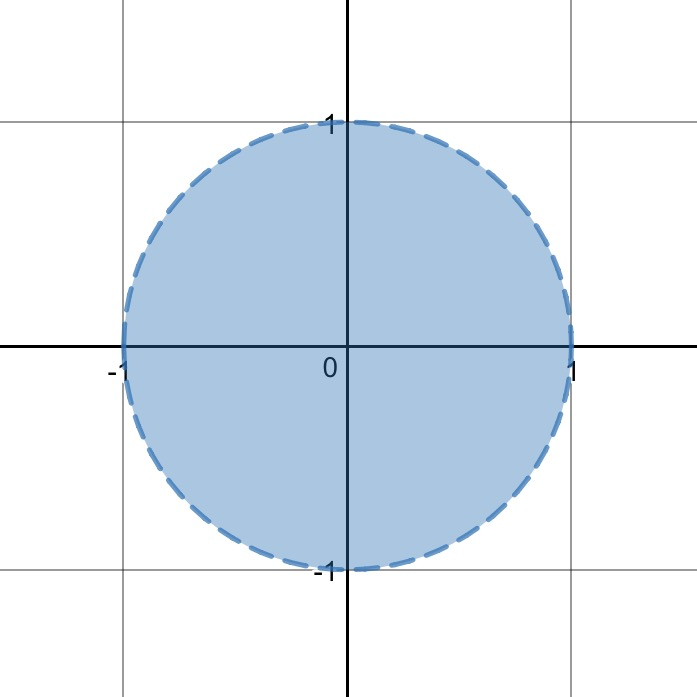
\includegraphics[scale=.125]{450b_hw3_prob4b_0}
%\caption{The set $U$ in $\R^2$}
%\end{figure}

Now, under $f$, every ordered pair maps either to itself, or to a corresponding ordered pair in the first quadrant (or on its boundary); so the image of $U$ is $f(U)=U\cap I$, where $I$ denotes the closure of the first quadrant.

\jpg{scale=.125}{450b_hw3_prob4b_1}

%\begin{figure}[h]
%\centering
%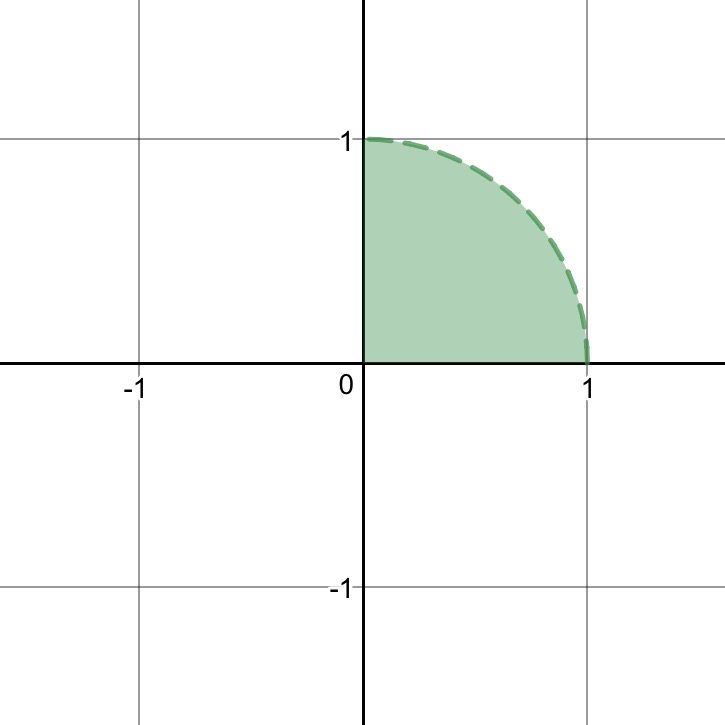
\includegraphics[scale=.125]{450b_hw3_prob4b_1}
%\caption{The set $f(U)$ in $\R^2$}
%\end{figure}

The set $f(U)$ is not open; since the origin $\vecb{0} \in f(U)$, but every $B(\vecb{0},r)$ contains points in every quadrant, so no open ball $B(\vecb{0},r)$ is a subset of $f(U)$.

\jpg{scale=.125}{450b_hw3_prob4b_2}

%\begin{figure}[h]
%\centering
%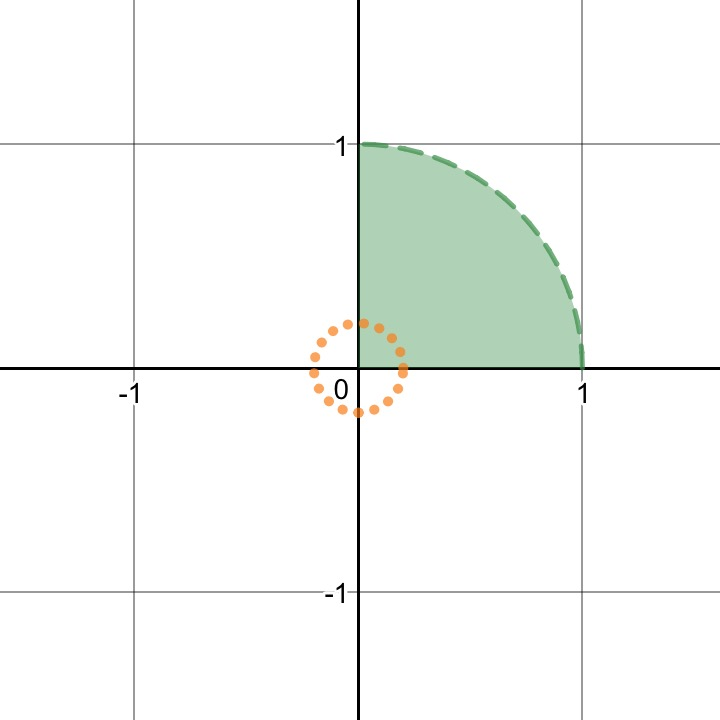
\includegraphics[scale=.125]{450b_hw3_prob4b_2}
%\caption{Every $B(\vec{0},r) \not\subset f(U)$}
%\end{figure}

Therefore, (2) fails. Thus, (1) $\centernot\implies$ (2). 
\end{proof}
\end{example*}

%6
\item Suppose that  $f:A\subset \R^n\to \R$ is continuous, with $\vecb{a}\in A$ and $f(\vecb{a})>0$. Prove that there exists a $\delta>0$ such that $f(\vecb{x})>0$ for all $\vecb{x}\in B(\vecb{a},\delta)\cap A$. 
\begin{proof}
Since $f$ is continuous on $A$, for every $\epsilon>0$, there exists a $\delta>0$ such that if $\norm{\vecb{x}-\vecb{a}}<\delta$ and $\vecb{x}\in A$, then $\norm{f(\vecb{x})-f(\vecb{a})}<\epsilon$. Let $\epsilon=f(\vecb{a})$. If $\norm{f(\vecb{x})-f(\vecb{a})}<f(\vecb{a})$, then $f(\vecb{x})\in B(f(\vecb{a}), f(\vecb{a}))$, which is the interval $(0, 2f(\vecb{a}))$. Thus, we are done.
\end{proof}

%7
\item Suppose that $A \subset \R^n$ is a set which is not closed. Prove that there exists a continuous function $f:A\to\R$ which is unbounded. (Hint: You might find it useful to first show that the set $\R^n-A$ must contain a point in the boundary of $A$.)
\begin{lemma*}[7.1]
If a set $A$ contains all its boundary points, then it is closed. 
\end{lemma*}
\begin{proof}
$A$ contains all of its boundary points, so $A^\complement$ contains none of them. That is, for all $\vecb{x}\in A^\complement$, $\vecb{x}$ is not a boundary point, so there exists some $r>0$ such that $B(\vecb{x}, r)\subset A^\complement$. This means that $A^\complement$ is open, by the openness criterion. Furthermore, since $A^\complement$ is open, $A$ is closed. 
\end{proof}
By the way, we have also proved the following:
\begin{corollary*}[7.2]
If a set $A$ contains none its boundary points, then it is open.
\end{corollary*}
Okay, now we are ready to prove Exercise 7. 
\begin{proof}
Suppose that $A \subset \R^n$ is not closed. By the contrapositive of Lemma (7.1), $A$ does not contain all of its boundary points. Let $\vecb{p}$ be a boundary point of $A$ which is not in $A$. Now, let $f:A\to\R$ be defined as 
$$f(\vecb{x})=\frac{1}{\norm{\vecb{x}-\vecb{p}}}.$$
To see that $f$ is unbounded, observe that for any $B>0$, $B(\vecb{p},\frac{1}{B})$ contains a point in $A$, so there exists some $\vecb{a}\in B(\vecb{p},\frac{1}{B})$ such that $\norm{\vecb{a}-\vecb{p}}<\frac{1}{B}$, so $f(\vecb{x})=\frac{1}{\norm{\vecb{a}-\vecb{p}}}>B$. 
\end{proof}
\end{enumerate}

\end{document}
